\documentclass{article}
\usepackage[utf8]{inputenc}
\usepackage[a4paper,top=2cm,bottom=2cm,left=3cm,right=3cm,marginparwidth=1.75cm]{geometry}
\usepackage{amsmath}
\usepackage{graphicx}
\usepackage[colorlinks=true, allcolors=blue]{hyperref}

\begin{document}

\begin{titlepage}

\center % Center everything on the page

\newcommand{\HRule}{\rule{\linewidth}{0.4mm}} % Barra horizontal

\begin{figure}[h]
    \centering
    
\includegraphics[width=0.24\linewidth]{images/uniMinho.jpg}
\end{figure}

%\textsc{\Large Universidade do Minho}\\[0.75cm]  % Name of your university/college
\textsc{\Large Licenciatura em Ciências da Computação}\\[0.4cm] % Nome do curso
\textsc{\Large Sistemas de Comunicações e Redes}\\[5cm]

{\Large\bfseries Ensaio Escrito}\\[0.5cm]
{\LARGE \bfseries Aplicações e Camada de Transporte} % Título


\vspace{5cm} % Autores
{\bfseries Grupo 28} \\ \vspace{3mm}
Davide Santos (A102938) \\ \vspace{3mm}
Edgar Araújo (A102946) \\ \vspace{3mm}
Pedro Augusto Camargo (A102504) \\ \vspace{3mm}
\vspace{0.2cm}
{Novembro 2023}\\[0.2cm] % Data

\vfill % Fill the rest of the page with whitespace
\end{titlepage}

\tableofcontents
\pagebreak

\section{Nível aplicacional}
\subsection{Identifique o endereço IP da estação que formulou a query DNS e o tipo de query realizada.}
\begin{figure}[h]
    \centering
    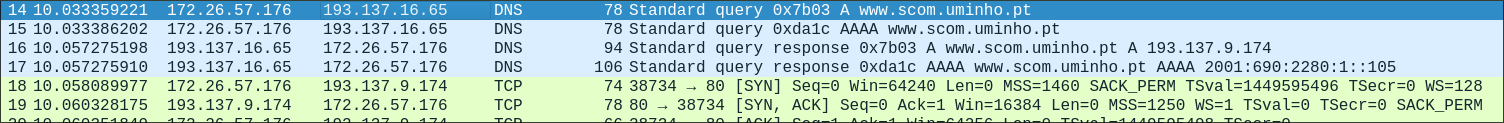
\includegraphics[width=1\linewidth]{images/dns.png}
\end{figure}

O endereço IP da estação que formulou a query DNS: 172.26.57.176 (O meu computador)
Foram enviadas 2 querys dns, uma do tipo A (endereço IPv4) e outra do tipo AAAA (endereço IPv6)

\subsection{Localize a trama com a resposta à query DNS formulada. Identifique nesta trama o endereço IP do
servidor web. Identifique também o servidor de nomes que forneceu a resposta, através do seu IP e nome}

\end{document}
